\documentclass[journal]{IEEEtran}
\usepackage{cite}
\usepackage{amsmath}
\usepackage{listings}
\usepackage{courier}
\usepackage{cuted}
\usepackage{graphicx}
\usepackage[hidelinks]{hyperref}
\usepackage{tabularx}
\usepackage{cleveref}

\lstset{basicstyle = \ttfamily, breaklines = true}

\begin{document}

\title{Real-time Chord Recognition}
\author{Adam Belhouchat, Ashish Sareen}
\maketitle

\begin{abstract}
    Blahdy blah.
\end{abstract}
\begin{IEEEkeywords}
    chord, octave, chord recognition, chroma features, pitch class profile, pattern matching, cosine similarity, filter, downsampling, FFT, LCDK
\end{IEEEkeywords}

\section{Introduction}
\subsection{History with References}
Automatic chord recognition (ACR) is the process of determining what chord is being played given an audio sample, labelling the audio sample over time with the appropriate chord \cite{stark}.
A chord here is defined as two or more notes being played at the same time or close together \cite{cho}.
Chord recognition has many applications, such as music segmentation or determining the similarity between two music samples \cite{lee}, but one of the most attractive applications is in automatic transcription.
Manual transcription can be tedious and difficult, and automatic chord recognition systems can help musicians work more quickly and more accurately \cite{mauch_thesis}.
Because of its wide range of applications, chord recognition has been the subject of much research in the past few decades, trying to improve the number of chords it can recognize and its accuracy through novel methods and approaches \cite{pauwels}.

One of the first ACR systems was developed by Takuya Fujishima in 1999 \cite{pauwels}.
He used the discrete Fourier transform (DFT) of a music sample to generate a pitch class profile, also known as chroma feature or chroma vector, which encodes the harmonic information of the sample over twelve different pitch classes.
The chroma feature is then compared the templates, one for each of 27 different chords, and the closest match is chosen as the chord label in a process called pattern matching \cite{fujishima}.

Since then, chord recognition has evolved greatly.
Pattern matching is simple and effective, but it is not the most accurate \cite{jiang}.
Some researchers have found great success using hidden Markov models (HMMs) rather than template matching to perform ACR \cite{sheh}, and others have explored the use of deep learning and neural networks both to detect chords \cite{boulanger} and to extract features from the audio sample \cite{korzeniowski}.
However, both HMMs and deep learning require a significant amount of training data, and good training data may be difficult to come by.
Manual transcription is prone to errors due to human subjectivity \cite{pauwels} and as mentioned before, it can be time consuming.
Nevertheless, these approaches do show significant accuracy improvements over pattern matching \cite{jiang, boulanger}.
Each of these approaches has its pros and cons, and which one is most fitting depends on the specific application.


\subsection{Global Constraints}
The main constraints dealt with are the hardware limitations of the TI LCDK platform, which is an all-in-one microcontroller (MCU) with digital signal processor (DSP) and ARM processor (CPU), and other common peripheral components \cite{lcdk}.
The entire system is built around the operation of the LCDK unit.
The two major limitations are the memory size and processor speed.
The memory specifications are 128 MB SDRAM and 128 MB NAND Flash \cite{lcdk}.
The processor speed is listed as 456 MHz for both the DSP and CPU \cite{lcdk}.

These hardware constraints pose implications on the software needed to build the system.
The LCDK board is programmed using the TI Code Composer Studio (CCS) IDE in the C programming language \cite{lcdk}.
The memory constraints imply that the program’s memory allocation must be limited to prevent data overflow.
To that end, memory is dynamically allocated when needed and freed immediately after use with the in-built C \texttt{malloc()} and \texttt{free()} functions.
Since this is a real-time system, the processor speed places a constraint on the execution time of the program.
The system leverages the interrupt service routine (ISR) to take audio samples at the sample rate equal to 16000 Hz.
The interrupt loop in the code must have an execution time less than 62.5 microseconds in order to guarantee that samples are taken properly.
Functions that take a long time to complete, such as \texttt{fprintf()}, are used only at the end of the program when the real-time component is complete.


\section{Motivation}
One shortcoming of many modern chord recognition systems is the vast amount of data required to train these systems \cite{pauwels}.
As mentioned earlier, large datasets of accurately transcribed music are not easy to find, so we wanted to develop a system that would work without training.
Additionally, these data-driven approaches are opaque and it is difficult to understand how they determine the chords in an audio sample \cite{pauwels}.
Part of our motivation for pursuing this project was to increase our skills in real-time digital signal processing and to understand how automatic chord recognition works.
Throwing data at a neural network until it works does not help us understand chord recognition.

Another shortcoming of HMMs and neural networks is they are often more computationally expensive than pattern matching \cite{stark}.
They work well when a music sample has been prerecorded and is later fed into the system, but they are not fast enough to perform chord recognition and transcription in real-time.
We wanted to make a chord recognition system that would record musical chords and transcribe them in real-time, so we needed to approach our system differently from most modern systems.

Lastly, as mentioned earlier, we chose this project to learn more about real-time digital signal processing (DSP) and to gain more experiences with different applications of it.
Chord recognition requires many DSP techniques, including sampling a signal, processing it to extract features, performing some evaluation on those features, and then returning the results of that evaluation to the user \cite{fujishima}.
This project would give us valuable experience with all the important elements of DSP with the added constraint of performing it in real-time.
This required us to perform memory management and pay close attention to our code to make sure all functions were optimized, which are valuable skills for embedded software development.


\section{Approach}
\subsection{Team Organization}
The team for the project consisted of two people, and the majority of the work was done together in the lab during lab time.
Having two people worked well, because we could split up the work into its natural software and hardware components.
A typical workflow would have one person controlling the software of the LCDK with CCS and the other monitoring the interfaces, such as microphone and speakers, to the LCDK.
The software person would write code and run it on the LCDK.
The hardware person would be responsible for testing the program by giving the microphone input through recorded or live chord sequences.
Being able to incrementally test units in this fashion enabled us to quickly develop and debug our code.
We were generally successful at managing our time, utilizing the full extent of our given lab time and not needing to come in after hours.
With proper time management and team organization, we were able to accomplish our main goals.


\subsection{Plan and Implementation}
Our initial plan was as follows:

\subsubsection*{Weeks 1--2}
Find and format data.
Find a data set of various guitar chords.
Format data into frames.

\subsubsection*{Weeks 3--4}
Generate chroma features.
Test feature extraction in MATLAB.
Implement final version of feature extraction on LCDK.

\subsubsection*{Weeks 5--7}
Perform chord recognition on chroma features.
Test different classification algorithms (template, HMM, linear classifier, etc.) in MATLAB and find the best (most accurate) one.
Implement final classification algorithm on LCDK.

\subsubsection*{Weeks 8--9}
Test chord recognition (all on LCDK).
Test on data set.
Test on live performance.
Write output to console.

\subsubsection*{Weeks 9--10}
Write chord sequences to a file.
Write a plain text file for testing.
Write to standard format (guitar tabs, sheet music, etc.).

Our actual implementation went as follows:

\subsubsection*{Weeks 1--2}
We found several potential data sets from which samples were taken.
Then, we were able to construct a data set with several audio samples for each of the 24 chords that were implemented.

\subsubsection*{Weeks 3--4}
Instead of MATLAB, we used Python to prototype chroma feature extraction.
Python had an up-to-date library for chroma processing, and was easier to use than MATLAB \cite{librosa}.
Referring to this library and another paper, we were able to implement feature extraction on the LCDK \cite{librosa, stark}.

\subsubsection*{Weeks 5--7}
Instead of beginning with Python or MATLAB, we started developing on the LCDK to save time.
Our first attempt was to adapt a template-matching algorithm, which ended up working very well \cite{stark}.
It was the simplest to implement and had the lowest computational complexity.
We ended up not having to attempt any of the other classifiers, which included linear classifiers, HMM, and SVM.

\subsubsection*{Weeks 8--9}
We tested chord recognition by playing sequences of guitar chords and recording the classification accuracy.
We were pleased to find that when played live, the program was able to classify all of the chords.

\subsubsection*{Weeks 9--10}
We were able to write the sequences to a text file by assigning timestamps for the duration that a chord was played.
We did not get to our stretch goal, which was to write the sequence to a standard format.


\subsection{Standard}
The most common features used in automatic chord recognition systems are chroma features \cite{cho_chroma}.
First introduced by Fujishima, chroma features represent the pitch content of a music sample.
Basic chroma features are calculated by summing the magnitude of the DFT of the music signal over certain frequency bins \cite{fujishima}.
These bins correspond roughly to the energy in different pitch classes, such as C or G\#.
Each chroma vector has twelve elements, one for each note in an octave, corresponding to the twelve pitch classes that the frequency bins are mapped to, and the distribution of energy across the twelve pitch classes is used to determine which chord was played in the music sample \cite{jiang}.
Because of how ubiquitous and useful chroma features are in chord recognition, we chose to use them as our features for chord recognition.

To actually determine what chord the chroma features corresponds to, we use pattern matching, which is one of the most common methods of determining chords \cite{cho_chroma}.
In particular, we use binary pattern matching, where each chord has a corresponding template which is a specific arrangement of zeros and ones.
Since the chroma vector represents the pitch content of a music sample, we can create ideal template vectors that represent what the pitch content of a pure chord would look like.
For example, the template vector for the major C chord would be $\mathbf{v}_C = (1, 0, 0, 0, 1, 0, 0, 1, 0, 0, 0, 0)$, where the ones are where a major C should have pitch contributions and the zeros are pitches that should not be present in a major C.
In general, the tones that should be present in the ideal chord are one, while all the other tones are zero \cite{cho_chroma}.
To find the matching template, many implementations look for the minimum Euclidean distance between a template and the chroma feature \cite{stark}, but other approaches such as finding the minimum angle between the two are also used \cite{jiang}.
We chose to go with this latter approach as it gave us slightly better accuracy when testing.


\subsection{Theory}
The key mathematical elements of our chord recognition system are the low-pass filter, the chroma features, and pattern matching.
In this section, we will explain in detail the theory behind each of these steps.

The low-pass filter is generated using the bilinear transform, which converts a continuous transfer function to a discrete one.
To do so, the bilinear transform uses the approximate map
\begin{equation}
    s \to \frac{2}{T}\frac{1 - z^{-1}}{1 + z^{-1}}
    \label{eq:s_to_z}
\end{equation}
where T is the sampling period of the discrete signal.
We can then substitute this into the continuous transfer function $H_a(s)$ to get the discrete one $H_d(z)$ by 
\begin{equation}
    H_d(z) = H_a\!\left(\frac{2}{T}\frac{1 - z^{-1}}{1 + z^{-1}}\right)
    \label{eq:bilinear}
\end{equation}
Once we have $H_d(z)$, we can get the discrete time-domain equation by partial fractions and inverse Z-transform pairs.

We used a 6th order Butterworth low-pass filter with a cutoff frequency at 6000 Hz.
This cutoff frequency preserved most of the important harmonic information while still filtering out high-frequency noise, and the order gave a reasonably steep dropoff around the cutoff frequency without being computationally expensive.
The actual transfer function is too large and complex to show here, so we used a program to generate the time-domain filter function.
The frequency response is given in \Cref{fig:frequency_response}.

\begin{figure}[t]
    \centering
    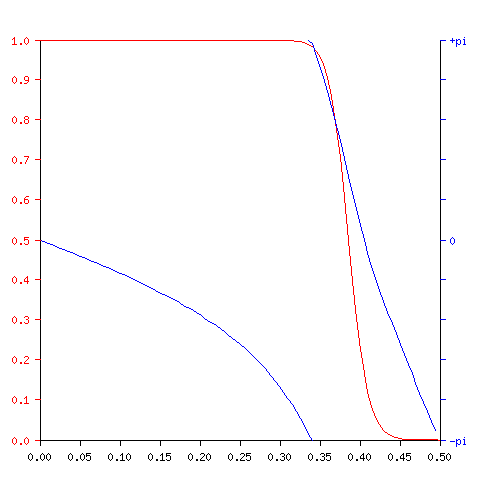
\includegraphics[width=\linewidth]{../Figures/frequency_response}
    \caption{Frequency response of the low-pass filter used in our chord recognition system.
    The red curve is the normalized magnitude of the frequency response and the blue curve is the phase.
    Generated from Tony Fisher's website at \url{https://www-users.cs.york.ac.uk/~fisher/mkfilter/}.}
    \label{fig:frequency_response}
\end{figure}

Chroma features are features that describe the pitch content of a sample of music \cite{jiang}.
A chroma feature has 12 elements, one for each note in an octave from C through B.
The value of one of these elements corresponds to the energy present in the music signal coming from that pitch.
Because of this, it is straightforward to determine the chords in a piece of music by analyzing the chroma features.

The algorithm we use to generate chroma features comes from Stark and Plumbley’s paper \cite{stark}.
The first step is to apply a Hamming window $w(n)$ to the signal $x(n)$, given by
\begin{equation}
    w(n) = 0.54 - 0.46\cos\!\left(\frac{2\pi n}{N - 1}\right)
    \label{eq:window}
\end{equation}
where $N$ is the size of the signal.
Once we have the windowed signal $x_w(n) = x(n)w(n)$ we take the DFT,
\begin{equation}
    X(k) = \sum_{n = 0}^{N - 1}x_w(n)e^{-\frac{i2\pi kn}{N}}
    \label{eq:dft}
\end{equation}

From here, the original chroma feature algorithm would sum the squared magnitudes of the DFT over certain frequency bins to get the chroma values \cite{fujishima}.
However, this may include unwanted energy like noise in the chroma features.
To avoid this, Stark and Plumbley only consider the maximum amplitude in a given frequency bin, thus only taking into account the energy in the note we want.

First, we determine the frequencies to search over.
We start with $f_{\text{C}3} = 130.81$ Hz, which is lower C.
Then for $n = 0, 1, \ldots, 11$, we calculate
\begin{equation}
    f(n) = f_{\text{C}3}2^{(n / 12)}
    \label{eq:freq}
\end{equation}
which gives the 12 notes in an octave.
We then do this for two octaves so we get all 24 notes in the two octaves from $f_{\text{C}3} = 130.81$ Hz to $f_{\text{C}5} = 523.25$ Hz.
For each of the 12 elements of the chroma feature, we search through two octaves and within each octave search through two harmonics.
This is because Stark and Plumbley have found that most instruments of interest use the lower register within this frequency range and to account for inharmonicities in real instruments \cite{stark}.
The chroma feature is then given by
\begin{equation}
    c_n = \frac{1}{h}\sum_{\phi = 1}^2\sum_{h = 1}^2 \max_{k_0^{(n, \phi, h)} \leq k \leq k_1^{(n, \phi, h)}} X(k)
    \label{eq:chroma}
\end{equation}
where $c_n$ are the elements of the chroma vector $\mathbf{c}$, $n = 0, 1, \ldots, 11$, $\phi$ is the number of the octave, $h$ is the number of the harmonic, and 
\begin{equation*}
    k_0^{(n, \phi, h)} = k'^{(n, \phi, h)} - rh
\end{equation*}
\begin{equation*}
    k_1^{(n, \phi, h)} = k'^{(n, \phi, h)} + rh
\end{equation*}
where $r = 2$ is the number of bins to search over for each harmonic and 
\begin{equation*}
    k'^{(n, \phi, h)} = \text{round}\!\left(\frac{f(n)\phi h}{f_s / N}\right)
\end{equation*}
where $f_s$ is the sampling rate.

Lastly, we use pattern matching to match the chroma feature to the most fitting chord.
Pattern matching involves the use of template vectors for each chord, such as $\mathbf{v}_{\text{C}} = (1, 0, 0, 0, 1, 0, 0, 1, 0, 0, 0, 0)$ for major C \cite{jiang}.
We try to match the chroma vector to the closest template vector and from that get the corresponding chord.
One simple method is to just find the Euclidean distance $||\mathbf{c} - \mathbf{v}||$ between the chroma vector and each of the template vectors and see which is the smallest.
Another approach, which we use,  is to find the cosine similarity between two vectors, defined as 
\begin{equation}
    \text{cossim}(\mathbf{c}, \mathbf{v}) = \frac{\langle\mathbf{c}, \mathbf{v}\rangle}{||\mathbf{c}|| \cdot ||\mathbf{v}||}
    \label{eq:cossim}
\end{equation}
and choose the template vector with the maximum cosine similarity \cite{jiang}.


\subsection{Software/Hardware}
There were two main types of software used for the project: the LibROSA Python package for prototyping, and Code Composer Studio (CCS) C software for implementation.
The LibROSA Python package was used in the early stages of development for chroma feature extraction.
The main motivation was to familiarize ourselves with the chroma structure and the type of inputs/outputs that our program would need.
The LibROSA package also provided functions to visualize the contents of a chroma feature, which helped to further understand the nature of the audio transformation.
After using this package, we were able to better organize our C code for the LCDK, keeping in mind its real-time constraints.

The majority of the software was done in Code Composer Studio in order to program the LCDK.
We were familiar with CCS since we used it extensively in prior projects.
The main challenge was to adapt the chroma feature extraction and chord recognition into the C programming language, which requires more low-level knowledge than Python.
Fortunately, with prior experience in C/C++ and relative simplicity of the algorithms used, we were able to quickly implement our program.
An example code snippet from the chroma feature extraction, containing the \texttt{process\_audio\_frame()} function, found in \texttt{chromagram.h}, is provided in \Cref{code:audio} at the end of this report.

As aforementioned, the LCDK platform is the embedded system on which the compiled C program operates.
The main subsystems used were the CPU and DSP, memory, and audio codec.
The audio codec was easy to use, since the manufacturer provided the encapsulated functions needed to sample and save audio information to the C built-in data types.
Encapsulation enabled us to use the hardware without needing to know many of its low-level details and instead use our knowledge of the software.


\subsection{Operation}


\subsubsection{How the System was Built}
\begin{figure}[!t]
    \centering
    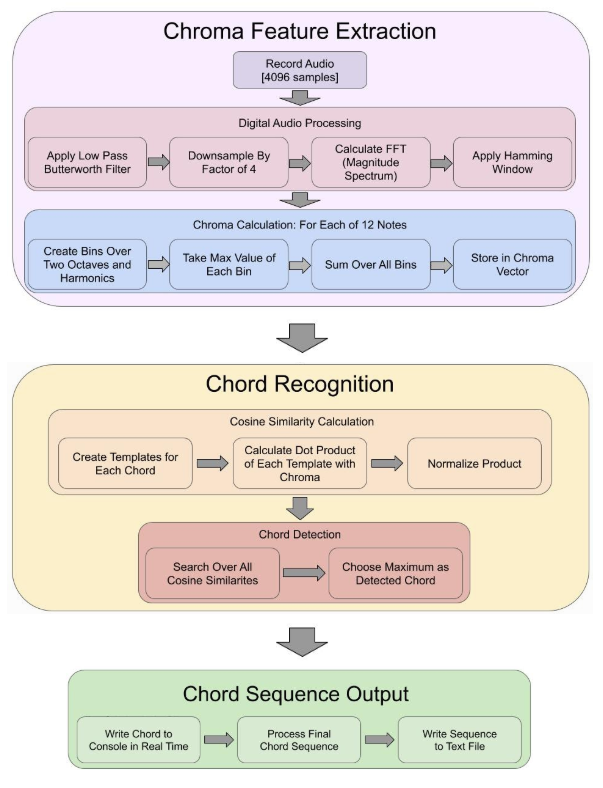
\includegraphics[width = \linewidth]{../Figures/block_diagram}
    \caption{Block diagram of the system.
    There are three main steps: chroma feature extraction, chord recognition, and chord sequence output.}
    \label{fig:block}
\end{figure}


\subsubsection{How to Use the System}
To use the chord recognition system, first plug a microphone into the LCDK microphone input port and plug speakers into the LCDK output port.
If you want, you can change the sampling rate, frame size, buffer size, and how long the program runs for.
The first three parameters are defined in \texttt{chromagram.h}: \texttt{FS} is sampling rate, \texttt{FRAME\_SIZE} is frame size, and \texttt{BUFFER\_SIZE} is buffer size which is fed into the FFT.
Note that \texttt{FRAME\_SIZE} must be a power of 2 and \texttt{BUFFER\_SIZE} must be one-fourth of \texttt{FRAME\_SIZE} due to the downsampling.
We choose to define them separately just to save that little bit of processing power required to perform the division by four.
The program length is implicitly defined by \texttt{ITERATIONS} in \texttt{main.c}.
Strictly speaking, it controls how many loops the program will run for, which is also the number of chords that will be processed.

Once all the parameters are set to your liking, run the program through Code Composer Studio and you will hear the “metronome” start to play through the speakers.
The metronome is really just a square wave that plays on beat to when the recording starts.
Once you hear the metronome, you can begin playing your audio samples into the microphone.
For best results, play the chords in time with the metronome, because otherwise the chord will be out of sync with the recording and the performance of the chord recognition system will be poor.

Once you start the program, the system will write the chords it has recognized to console.
The most recent message will be the chord that was just played and recorded.
Once the program has run through all iterations, it will print ``Done :)'' at which point you will find a file named \texttt{chord\_sequence.txt} in the Debug folder.
This prints out all the chords that were played during recording along with the times that the chord was played.


\section{Results}

\begin{figure}[!t]
    \centering
    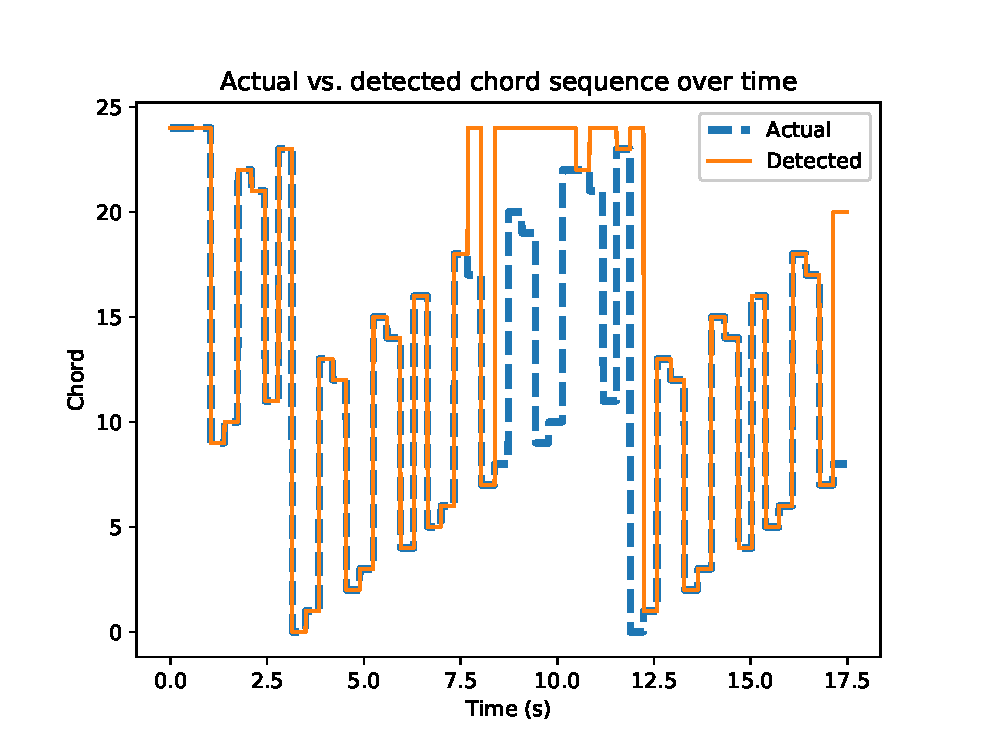
\includegraphics[width = \linewidth]{../Figures/chord_sequence_in_order}
    \caption{Graph of the performance of the system for a naturally ordered chord progression.}
    \label{fig:in_order}
\end{figure}
\begin{figure}[!t]
    \centering
    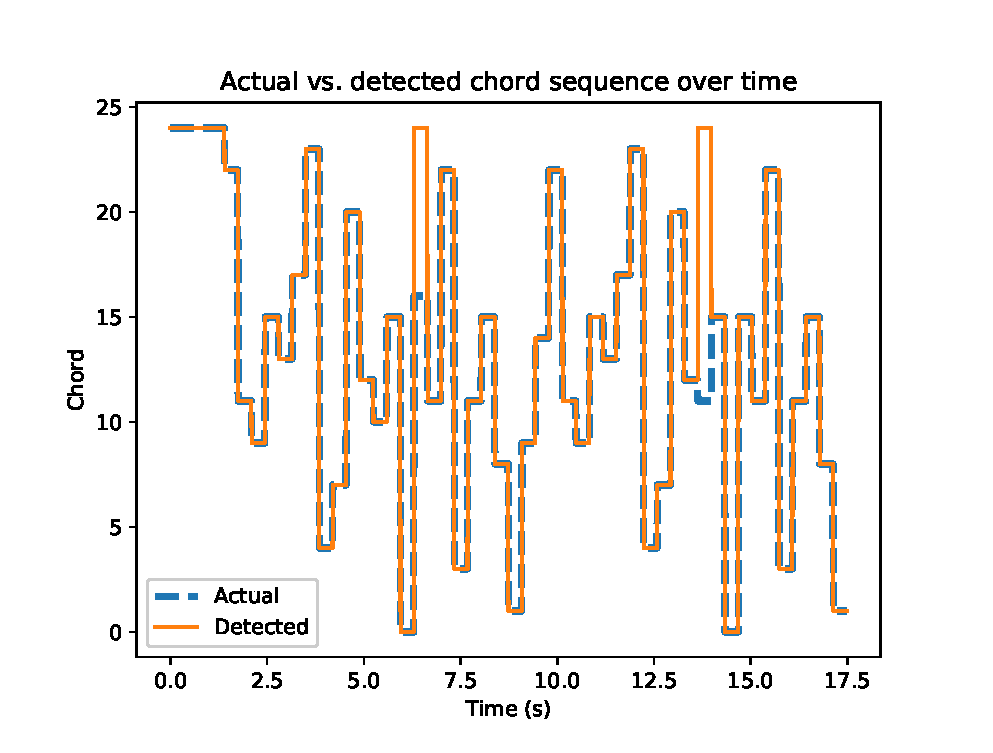
\includegraphics[width = \linewidth]{../Figures/chord_sequence_random}
    \caption{Graph of the performance of the system for a randomly ordered chord progression.}
    \label{fig:random}
\end{figure}


\subsection{Description}
We graphed the performance of our chord recognition system over two different chord sequences, one ordered naturally in \Cref{fig:in_order} and one ordered randomly in \Cref{fig:random}.
We follow the graph convention described by \cite{harte}, where the 24 chords from C major to B minor are numbered 0 to 23, with no chord assigned 24, and we plot the number of each chord over time.


\subsection{Discussion}


\bibliographystyle{IEEEtran}
\bibliography{refs}


\onecolumn
\begin{lstlisting}[language = C, frame = single, caption = {An example code snippet from the chroma feature extraction containing the \texttt{process\_audio\_frame()} function.
This function is located in the \texttt{chromagram.c} file.}, captionpos = b, label = code:audio]
void process_audio_frame(int16_t* input_audio_frame)
{
    /*
     * Processes the audio input and generates the chromagram.
     *
     * First downsamples the input audio signal and calculates 
     * the magnitude of the FFT, then generates the chromagram.
     */

    chroma_ready = 0;

    downsampled_audio_frame_size = FRAME_SIZE / 4;
    downsampled_input_audio_frame = (float*)
    malloc(downsampled_audio_frame_size * sizeof(float));
    downsample_frame(input_audio_frame);

    int i;
    for (i = 0; i < BUFFER_SIZE; i++)
    {
        x_sp[2 * i] = downsampled_input_audio_frame[i];
        x_sp[2 * i + 1] = 0;
    }

    free(downsampled_input_audio_frame);
    calculate_chromagram();
}
\end{lstlisting}


\end{document}